
\subsection{Diagramas de casos de uso}
Para ser possível visualizar graficamente todas as ações que os 
atores conseguem realizar e para melhorar a comunicação com as 
partes interessadas do projeto, foram desenvolvidos diagramas de 
casos de uso.

\subsubsection{Casos de uso Fórum}
Na imagem representada abaixo (Figura~\ref{fig:12}), é possível 
visualizar o diagrama de casos de uso para o fórum.
Neste, o técnico poderá ver as listagens de tópicos em destaque e tópicos mais recentes. Caso seja um técnico oficial terá acesso aos tópicos privados e os seus tópicos.
O técnico poderá também pesquisar por tópicos, dos quais ele terá a possibilidade de selecionar um para visualizar. 
O técnico conseguirá, além disso, criar um novo tópico, onde se dirigirá para a criação de tópicos. Aqui, o técnico será obrigado a inserir um título, descrição e tipo do tópico para o criar, 
mas poderá inserir imagens e indicar produto referente.
Para finalizar a criação o técnico conseguirá confirmar ou cancelar o processo. 

\begin{figure}[htb]
    \centering
    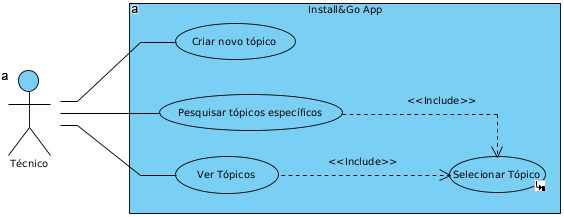
\includegraphics[width=0.6\textwidth]{images/diagramas/casos_de_uso/use_case_forum.png}
    \caption{Diagrama de casos de uso de fórum}
    \label{fig:12}
\end{figure}

\subsubsection{Casos de uso de pesquisar tópicos}

O técnico poderá realizar a pesquisa por tópicos específicos, 
esta será ser realizada por escrito onde indica o assunto a pesquisar e poderá ser filtrada.

O técnico terá também a possibilidade de pesquisar por código QR de produto, uma vez que, o servidor da Motorline esteja desenvolvido para tal.

\begin{figure}[htb]
    \centering
    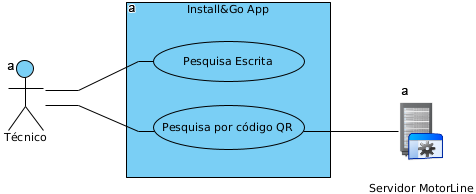
\includegraphics[width=0.6\textwidth]{images/diagramas/casos_de_uso/use_case_forum_search.png}
    \caption{Diagrama de casos de uso de pesquisa de tópicos}
    \label{fig:13}
\end{figure}

\subsubsection{Casos de uso ver detalhes de tópico}

Assim que um técnico seleciona um tópico, é movido para os 
detalhes, onde consegue visualizar os detalhes, responder e, caso seja o seu tópico, consegue finalizar, selecionar a melhor resposta, remover a melhor resposta, eliminar e alterar a visibilidade do tópico.

\begin{figure}[htb]
    \centering
    
    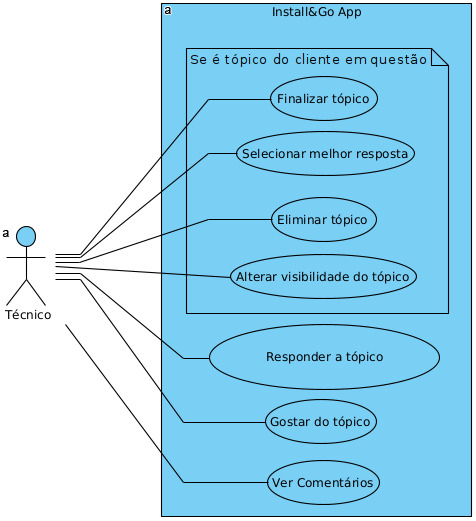
\includegraphics[width=0.5\textwidth]{images/diagramas/casos_de_uso/use_case_topic_details.png}
    \caption{Diagrama de casos de uso de detalhes de tópico}
    \label{fig:14}
\end{figure}

\subsubsection{Casos de uso ver comentários}

O técnico quando decide visualizar os comentários consegue responder e gostar de uma resposta ou comentário, caso este seja seu ainda o consegue apagar.

\begin{figure}[htb]
    \centering
    
    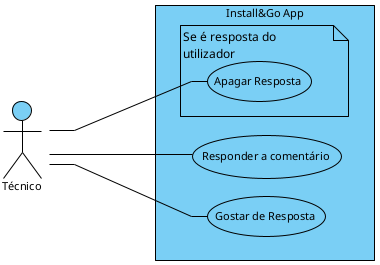
\includegraphics[width=0.5\textwidth]{images/diagramas/casos_de_uso/use_case_topic_comments.png}
    \caption{Diagrama de casos de uso de ver comentários}
    \label{fig:15}
\end{figure}

\subsubsection{Casos de uso ativação de conta}

Assim que uma conta é confirmada, um \textit{email} de ativação é enviado para técnico e esta deverá ser ativada.
Para isto, o código deverá ser indicado pelo técnico para se proceder à ativação da conta. Este, poderá em caso de necessidade, pedir o reenvio do código de ativação, o qual será gerado novamente e reenviado.

\begin{figure}[htb]
    \centering
    
    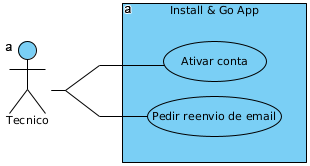
\includegraphics[width=0.5\textwidth]{images/diagramas/casos_de_uso/use_case_account_validation.png}
    \caption{Diagrama de casos de uso de ativação de conta}
    \label{fig:16}
\end{figure}

\subsubsection{Casos de uso perfil}

Sempre que o técnico desejar alterar alguma informação, este poderá alterar o seu nome, \textit{email} e imagem de perfil.

\begin{figure}[htb]
    \centering
    
    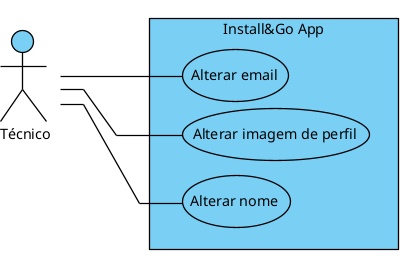
\includegraphics[width=0.5\textwidth]{images/diagramas/casos_de_uso/use_case_perfil.png}
    \caption{Diagrama de casos de uso de ativação de conta}
    \label{fig:17}
\end{figure}

\newpage

\subsubsection{Casos de uso notificações}

Sempre que o técnico desejar ver as suas notificações, poderá seleciona-las, também dispõe da possibilidade de alterar a configuração das notificações, para apenas as receber por \textit{email} ou push, ou então, ambas. Terá também a possibilidade de personalizar cada método, para receber um relatório diário de notificações ou então, notificações em tempo real.

\begin{figure}[htb]
    \centering
    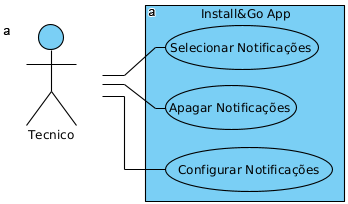
\includegraphics[width=0.5\textwidth]{images/diagramas/casos_de_uso/use_case_notificacoes.png}
    \caption{Diagrama de casos de uso de ativação de conta}
    \label{fig:18}
\end{figure}

\subsubsection{Casos de uso gestão de recursos humanos}

Uma empresa poderá registar contas para os seus técnicos no seu nome, com a indicação do \textit{email} e nºcontribuinte. Esta poderá também impedir acesso a estas contas ou remover completamente a conta da aplicação.

\begin{figure}[htb]
    \centering
    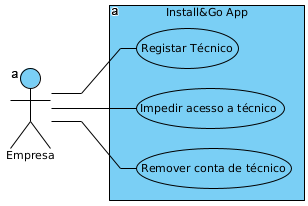
\includegraphics[width=0.5\textwidth]{images/diagramas/casos_de_uso/use_case_rec_humanos.png}
    \caption{Diagrama de casos de uso de ativação de conta}
    \label{fig:19}
\end{figure}